\section{Результати роботи та аналіз}

Тестування проводилось під Linux-based операційними системами на двох ПК. Перший ПК мав процесор Intel i5-2400 з заявленною тактовою частотою 3,1 ГГц. Другий ПК мав процесор AMD Sempron 2800+ з заявленною тактовою частотою 1,6 ГГц. 

Спершу розглянемо результати роботи бенчмарку при компіляції у 64-бітному режимі на ПК з процесором Intel:

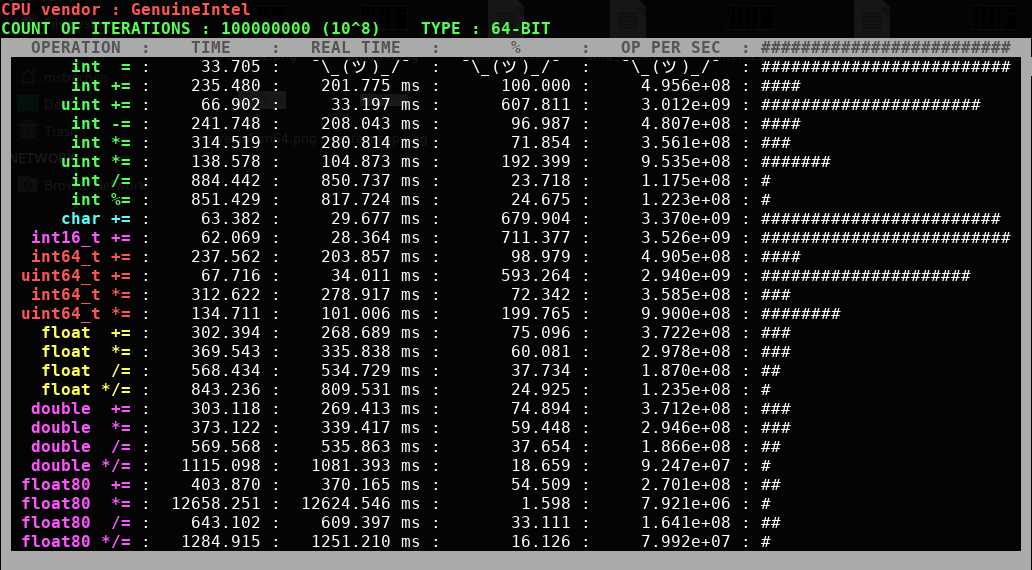
\includegraphics[width = 16cm]{img/intel64.png}

Як і очікувалось, різниці у часі між операціями над 64-бітними та 32-бітними цілочисельними типами даних немає.

Порівняємо з результатами роботи бенчмарку у 32-бітному режимі:

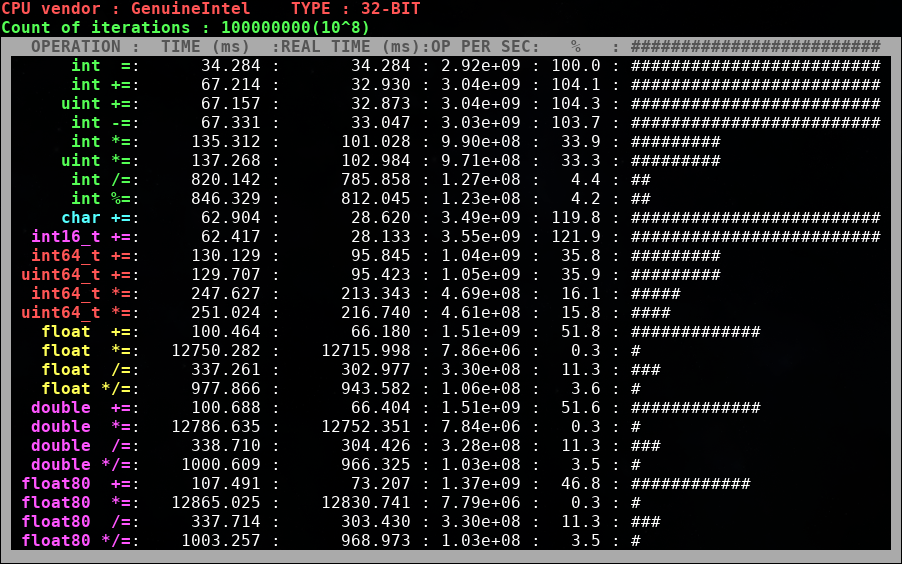
\includegraphics[width = 16cm]{img/intel32.png}

Бачимо, що операції над 64-бітними цілими стали коштувати приблизно вдвічі дорожче відносно 32-бітних цілих. Дуже неприємним моментом є погіршення опрацювання операції множення над дійсними числами. На це є дві причини. Першу причину можна помітити, проаналізувавши результати "просто множення" і "множення + ділення" над дійсними типами данних.  В данному бенчмарку є особливість - при множенні, починаючи з деякої ітерації ми отримуємо у змінній значення inf (через недосконалість збереження данних у цих типах даних). Через це страждає виконанн операції множення (тому що обробка "нескінченності" як окремого випадку займає додаткові ресурси процесора). 
Друга причина криється в особливостях компіляції. Проаналізуємо згенерований асемблерний код.

Ліворуч - вихідний текст на C++, по центру - згенерований код у випадку компіляції з прапорцем -m32, праворуч - у випадку компіляції з прапорцем -m64. 


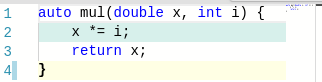
\includegraphics[width = 6cm]{img/screencpp.png}
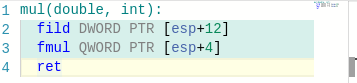
\includegraphics[width = 6cm]{img/screenAsm32.png}
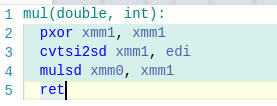
\includegraphics[width = 5cm]{img/screenAsm64.png}

Як бачимо, у випадку компіляції у 32-бітному режимі операції виконуються з оперативною пам'ятю, а ось у випадку 64-бітного режиму усе виконується виключно в регістрах. Регістри при цьому значно швидші за доступом, а тому вітка обробки нескінченних значень у типах з плаваючою комою виконується довше.

Тепер проаналізуємо швидкодію ПК з процесором AMD.

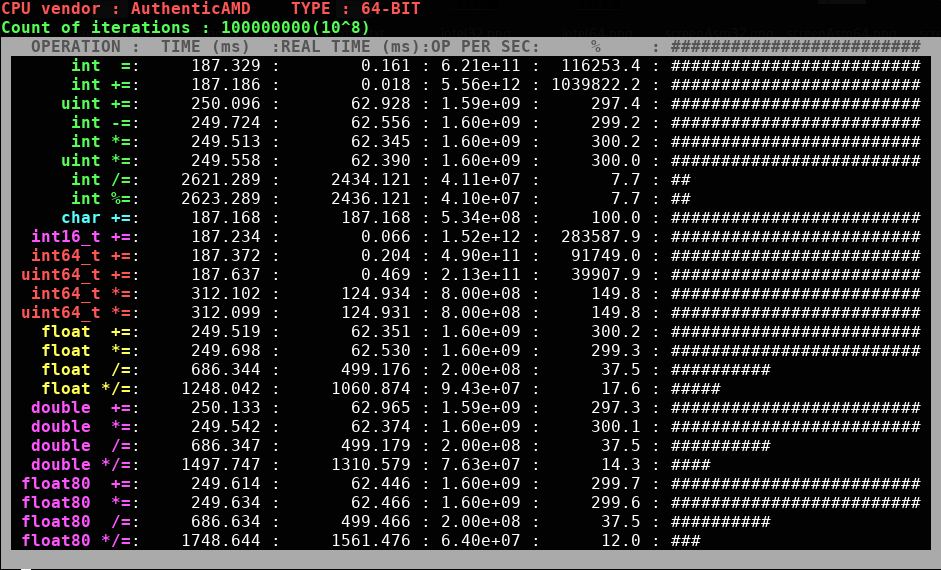
\includegraphics[width = 16cm]{img/amd64.png}

Якщо порівнювати з Intel, то процесор від AMD очевидно по-іншому діє з операціями над типами даних. У той час, коли у Intel операція \textbf{"int +="} займає приблизно вдвічі більше часу, ніж операція \textbf{"int ="}, то з в AMD ці дві операції майже однакові по часу. Можливо, процесор від інтел розділяє операцію  \textbf{"int +="} на дві, а AMD робить усе "на місці". 

Проаналізуємо також виконання бенчмарку з прапорцем -m32.

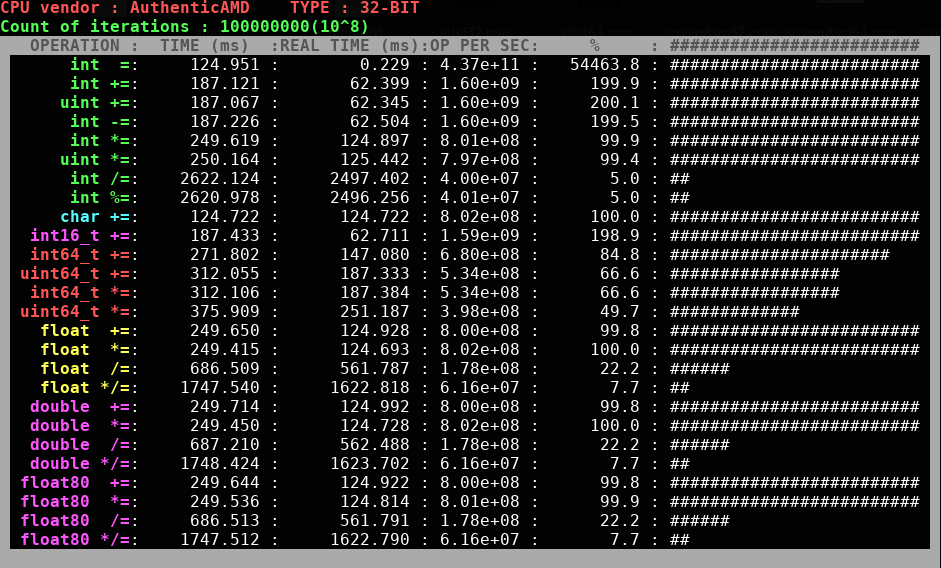
\includegraphics[width = 16cm]{img/amd32.png}
 
Помітна деградація у два рази в операціях над 64-бітними цілими, але загалом усе досить природньо (і немає неприємних особливостей при роботі з \textbf{INF} у дійсних типах, як у Intel).


